\documentclass[12pt,a4paper]{article}
\usepackage[utf8]{vietnam}
\usepackage{amsmath,amssymb}
\usepackage{geometry}
\geometry{
  top=12mm,
  bottom=12mm,
  left=14mm,
  right=14mm,
  footskip=6mm,
  headheight=14pt
}

\usepackage{tikz}
\usetikzlibrary{arrows.meta,calc,shapes.geometric}
\usepackage[most]{tcolorbox}
\usepackage{fontawesome}
\usepackage{fancyhdr}
\usepackage{enumitem}

\pagestyle{fancy}
\fancyhf{}
\fancyhead[L]{\footnotesize\color{teal!80!black}\faBook\ \textbf{SỔ TAY KIẾN THỨC TOÁN 3}}
\fancyhead[R]{\footnotesize\color{teal!80!black}\textbf{Lớp Toán Thầy Lĩnh -- loptoanthaylinh.vn}}
\fancyfoot[C]{\footnotesize\color{gray}-- Sổ tay kiến thức: Bài 11. Bảng nhân 8, bảng chia 8 --}
\renewcommand{\headrulewidth}{0.4pt}
\renewcommand{\footrulewidth}{0pt}

\setlength{\parindent}{0pt}
\setlength{\parskip}{0pt}

\begin{document}

% --- BANNER BÀI HỌC ---
\begin{tcolorbox}[
  enhanced,
  colback=teal!8!white,
  colframe=teal!70!black,
  arc=3mm, boxrule=1.2pt,
  left=3mm, right=3mm, top=2mm, bottom=2mm,
  halign=center
]
  {\LARGE\bfseries\color{teal!90!black}\faBookmark\ BÀI 11: BẢNG NHÂN 8, BẢNG CHIA 8}\\[1mm]
  {\itshape\footnotesize\color{black!75} Quy tắc đếm thêm 8, các tích chẵn tận cùng 0, 2, 4, 6, 8 trên 1 trang A4}
\end{tcolorbox}

\vspace{-2mm}

\noindent
\begin{minipage}[t]{0.49\textwidth}\vspace{0pt}
\begin{tcolorbox}[
  enhanced,
  colback=blue!4!white,
  colframe=blue!75!black,
  arc=2mm, boxrule=0.8pt,
  left=2mm, right=2mm, top=1.8mm, bottom=1.8mm,
  title={\footnotesize\bfseries\color{white}\faTimes\ 1. Bảng nhân 8 (Đếm thêm 8)}
]
{\footnotesize
\begin{itemize}\setlength{\itemsep}{0.6pt}\setlength{\leftskip}{-2.5mm}
  \item Dãy tích của bảng 8 tăng đều 8 đơn vị:
  $$8, 16, 24, 32, 40, 48, 56, 64, 72, 80$$
  \item Toàn bộ các tích đều là \textbf{số chẵn}.
  \item \textbf{Các mốc ghi nhớ quan trọng:}
  \begin{itemize}\setlength{\itemsep}{0.5pt}\setlength{\leftskip}{-2.5mm}
    \item $8 \times 5 = 40$ (Mốc số tròn chục).
    \item $8 \times 8 = \mathbf{64}$ (Hai số giống nhau).
    \item $8 \times 7 = 56$; $8 \times 9 = \mathbf{72}$.
  \end{itemize}
  \item Mẹo: Nhân với 8 là gấp đôi 3 lần liên tiếp ($k \times 2 \times 2 \times 2$).
\end{itemize}
}
\end{tcolorbox}
\end{minipage}
\hfill
\begin{minipage}[t]{0.49\textwidth}\vspace{0pt}
\begin{tcolorbox}[
  enhanced,
  colback=teal!4!white,
  colframe=teal!75!black,
  arc=2mm, boxrule=0.8pt,
  left=2mm, right=2mm, top=1.8mm, bottom=1.8mm,
  title={\footnotesize\bfseries\color{white}\faShareAlt\ 2. Bảng chia 8 (Từ nhân suy ra chia)}
]
{\footnotesize
\begin{itemize}\setlength{\itemsep}{0.6pt}\setlength{\leftskip}{-2.5mm}
  \item Lấy tích chia cho 8 thì được thừa số kia:
  \begin{tabular}{ll}
    $8 : 8 = 1$ & $48 : 8 = 6$\\
    $16 : 8 = 2$ & $56 : 8 = 7$\\
    $24 : 8 = 3$ & $64 : 8 = 8$\\
    $32 : 8 = 4$ & $72 : 8 = 9$\\
    $40 : 8 = 5$ & $80 : 8 = 10$
  \end{tabular}
  \item Muốn tính $72 : 8$, ta nhẩm: "Mấy nhân $8$ bằng $72$?". Vì $8 \times 9 = 72 \implies 72 : 8 = 9$.
\end{itemize}
}
\end{tcolorbox}
\end{minipage}

\vspace{-2.5mm}
% --- KHỐI 3: SƠ ĐỒ TƯ DUY TIKZ ---
\noindent
\begin{tcolorbox}[
  enhanced,
  colback=orange!4!white,
  colframe=orange!80!black,
  arc=2mm, boxrule=0.8pt,
  left=2mm, right=2mm, top=1.5mm, bottom=1.5mm,
  title={\footnotesize\bfseries\color{white}\faSitemap\ SƠ ĐỒ TƯ DUY: TIẾN TRÌNH DÃY TÍCH TĂNG DẦN CỦA BẢNG 8}
]
\centering
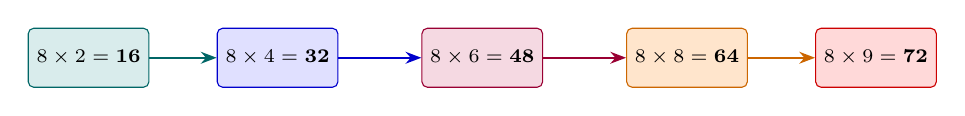
\begin{tikzpicture}[
  box/.style={draw, rounded corners=2pt, align=center, font=\scriptsize\bfseries, inner sep=3pt, minimum height=0.75cm},
  arr/.style={-{Stealth[length=2mm]}, thick}
]
  \node[box, fill=teal!15, draw=teal!80!black] (e1) at (0, 0) {$8 \times 2 = \mathbf{16}$};
  \node[box, fill=blue!12, draw=blue!80!black] (e2) at (2.4, 0) {$8 \times 4 = \mathbf{32}$};
  \node[box, fill=purple!15, draw=purple!80!black] (e3) at (5.0, 0) {$8 \times 6 = \mathbf{48}$};
  \node[box, fill=orange!20, draw=orange!80!black] (e4) at (7.6, 0) {$8 \times 8 = \mathbf{64}$};
  \node[box, fill=red!15, draw=red!80!black] (e5) at (10.0, 0) {$8 \times 9 = \mathbf{72}$};

  \draw[arr, teal!80!black] (e1) -- (e2);
  \draw[arr, blue!80!black] (e2) -- (e3);
  \draw[arr, purple!80!black] (e3) -- (e4);
  \draw[arr, orange!80!black] (e4) -- (e5);
\end{tikzpicture}
\end{tcolorbox}

\vspace{-2.5mm}
% --- KHỐI 4: VÍ DỤ & MẸO TRÁNH BẪY ---
\noindent
\begin{minipage}[t]{0.49\textwidth}\vspace{0pt}
\begin{tcolorbox}[
  enhanced,
  colback=green!4!white,
  colframe=green!60!black,
  arc=2mm, boxrule=0.8pt,
  left=2mm, right=2mm, top=1.8mm, bottom=1.8mm,
  title={\footnotesize\bfseries\color{white}\faCheckCircle\ Ví dụ thực hành chuẩn mực}
]
{\footnotesize
\textbf{1. Tính nhẩm:}\\
$8 \times 3 = \mathbf{24}$;\quad $8 \times 7 = \mathbf{56}$.\\
$64 : 8 = \mathbf{8}$;\quad $72 : 8 = \mathbf{9}$.\\
\textbf{2. Tìm $x$:}\\
$x \times 8 = 48 \implies x = 48 : 8 = \mathbf{6}$.\\
\textbf{3. Bài toán thực tế:}\\
Mỗi con nhện có $8$ cái chân. Hỏi $6$ con nhện có tất cả bao nhiêu cái chân?\\
\textit{Bài giải:} Số cái chân là: $8 \times 6 = \mathbf{48}$ (cái chân).
}
\end{tcolorbox}
\end{minipage}
\hfill
\begin{minipage}[t]{0.49\textwidth}\vspace{0pt}
\begin{tcolorbox}[
  enhanced,
  colback=red!4!white,
  colframe=red!70!black,
  arc=2mm, boxrule=0.8pt,
  left=2mm, right=2mm, top=1.8mm, bottom=1.8mm,
  title={\footnotesize\bfseries\color{white}\faExclamationTriangle\ Mẹo tránh bẫy trắc nghiệm}
]
{\footnotesize
\begin{itemize}\setlength{\itemsep}{1.5pt}\setlength{\leftskip}{-2.5mm}
  \item \textbf{Mẹo gấp đôi 3 lần:} Khi quên $8 \times 6$:\\
  Lấy $6 \times 2 = 12 \to 12 \times 2 = 24 \to 24 \times 2 = \mathbf{48}$. Cực kì nhanh và không thể sai!
  \item \textbf{Bẫy hay nhầm $8 \times 4$ và $8 \times 3$:}\\
  $8 \times 3 = 24$; $8 \times 4 = 32$. Nhớ chữ số hàng chục tăng dần: $24 \to 32 \to 40$.
\end{itemize}
}
\end{tcolorbox}
\end{minipage}


\end{document}
